% 2010 年上海春季卷第 13 题：斜截圆柱示意（底面直径 40 cm，母线最短 50 cm、最长 80 cm）。
% 来源 PDF：春季高考/2010/2010春季上海.pdf，SHA-256 24926e5272a6316cbaa399c0a097b3986ab34563db975016f98bae99f2274c56。
% 原页：第 1 页右栏中部（印刷页 2-37，《数学教学》2010 年第 2 期转载）。
% 重绘依据：圆柱下底为椭圆（上沿虚线、下沿实线），底面直径标 40 cm；
% 截口为倾斜椭圆，左母线 50 cm、右母线 80 cm 用双向箭头标注。
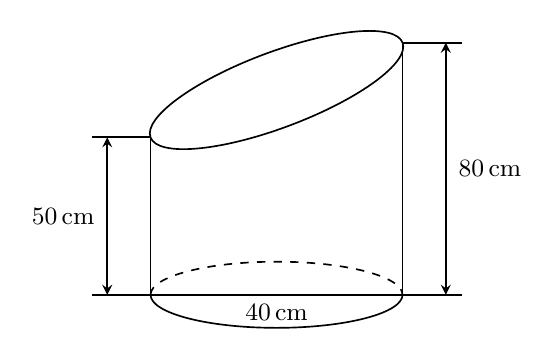
\begin{tikzpicture}[semithick, every node/.style={inner sep=1.5pt, font=\small}, >=stealth]
  % 下底椭圆：上半（背面）虚线，下半（正面）实线
  \draw[dashed] (-1.6,0) arc[start angle=180, end angle=0, x radius=1.6, y radius=0.42];
  \draw (-1.6,0) arc[start angle=180, end angle=360, x radius=1.6, y radius=0.42];
  % 底面直径
  \draw (-1.6,0) -- (1.6,0);
  \node at (0,-0.22) {$40\,\mathrm{cm}$};
  % 两条母线
  \draw (-1.6,0) -- (-1.6,2.0);
  \draw (1.6,0) -- (1.6,3.2);
  % 截口椭圆：两端点恰为两条母线的上端点 (-1.6,2.0) 与 (1.6,3.2)
  \draw[rotate around={20.6:(0,2.6)}] (0,2.6) ellipse (1.71 and 0.48);
  % 左侧 50 cm 标注
  \draw (-1.6,0) -- (-2.35,0);
  \draw (-1.6,2.0) -- (-2.35,2.0);
  \draw[<->] (-2.15,0) -- (-2.15,2.0);
  \node[left] at (-2.25,1.0) {$50\,\mathrm{cm}$};
  % 右侧 80 cm 标注
  \draw (1.6,0) -- (2.35,0);
  \draw (1.6,3.2) -- (2.35,3.2);
  \draw[<->] (2.15,0) -- (2.15,3.2);
  \node[right] at (2.25,1.6) {$80\,\mathrm{cm}$};
\end{tikzpicture}
